% README file for moduleDocumentationTemplate TeX template.
% This template should be used to document all Basilisk modules.
% Updated 20170711 - S. Carnahan
%
%-Copy the contents of this folder to your own _Documentation folder
%
%-Rename the Basilisk-moduleDocumentationTemplate.tex appropriately
%
% All edits should be made in one of:
% sec_modelAssumptionsLimitations.tex
% sec_modelDescription.tex
% sec_modelFunctions.tex
% sec_revisionTable.tex
% sec_testDescription.tex
% sec_testParameters.tex
% sec_testResults.tex
% sec_user_guide.tex
%
%-Some rules about referencing within the document:
%1. If writing the suer guide, assume the module description is present
%2. If writing the validation section, assume the module features section is present
%3. Make no other assumptions about any sections being present. This allow for sections of the document to be used elsewhere without breaking.

%In order to import some of these sections into a document in a different directory:
%\usepackage{import}
%Then, the sections are called with \subimport{relative path}{file} in order to \input{file} using the right relative path.
%\import{full path}{file} can also be used if absolute paths are preferred over relative paths.

%%%%%%%%%%%%%%%%%%%%%%%%%%%%%%%%%%%%%%%%%%%%%%%%%




\documentclass[]{BasiliskReportMemo}

\usepackage{cite}
\usepackage{AVS}
\usepackage{float} %use [H] to keep tables where you put them
\usepackage{array} %easy control of text in tables
\usepackage{graphicx}
\bibliographystyle{plain}


\newcommand{\submiterInstitute}{Autonomous Vehicle Simulation (AVS) Laboratory,\\ University of Colorado}


\newcommand{\ModuleName}{CSSWlsEst}
\newcommand{\subject}{Weight Least-Squares Minimum-Norm Coarse Sun Heading Estimator}
\newcommand{\status}{Released}
\newcommand{\preparer}{S. Piggott}
\newcommand{\summary}{This is a report documenting the results of the unit test performed for the 
   coarse sun sensor sun point vector estimation algorithm.  A weighted least-squares minimum-norm algorithm is used to estimate the body-relative sun heading using a cluster of coarse sun sensors.  Using two successive sun heading evaluation the module also computes the inertial angular velocity vector.  As rotations about the sun-heading vector are not observable, this angular velocity vector only contains body rates orthogonal to this sun heading vector.  }

\begin{document}

\makeCover

%
%	enter the revision documentation here
%	to add more lines, copy the table entry and the \hline, and paste after the current entry.
%
\pagestyle{empty}
{\renewcommand{\arraystretch}{2}
\noindent
\begin{longtable}{|p{0.5in}|p{3.5in}|p{1.07in}|p{0.9in}|}
\hline
{\bfseries Rev} & {\bfseries Change Description} & {\bfseries By}& {\bfseries Date} \\
\hline
1.0 & Initial Documentation & S. Piggott & 2016-10-01\\
\hline
1.1 & Modified Format to BSK documentation & H. Schaub & 2018-04-29\\
\hline
1.2 & Added User Guide Section & H. Schaub & 2018-04-29\\
\hline
1.3 & Added discussion on the inertial angular velocity vector evaluation & H. Schaub & 2018-05-26\\
\hline

\end{longtable}
}



\newpage
\setcounter{page}{1}
\pagestyle{fancy}

\tableofcontents %Autogenerate the table of contents
~\\ \hrule ~\\ %Makes the line under table of contents




\section{Introduction}
When in safe mode, the spacecraft uses its coarse sun sensors (CSSs) in order to 
point the vehicle's solar arrays at the Sun.  This is done in order to ensure 
that the vehicle gets to a power-positive state with a minimum set of sensors 
in order to recover from whatever event triggered the transition to safe mode.  
The nominal vehicle considered in this report has 8 coarse sun sensor (CSS) sensors available to it 
which allows it to resolve the exact sun direction in almost all body axes as 
long as all sensors are functional.  With these cosine CSS a minimum of 3 sensor must provide a signal to determine a unique answer.

\subsection{Sun Heading Evaluation}
If more than 3 CSS detect a sun signal, the algorithm needs to be able to obtain 
the sun pointing vector that best fits the current outputs from all of the CSSs.  
This is done by a least squares estimation process that provides the sun vector 
that best fits from a weighted least squares perspective.  The weights are 
simply set based on the current output of each sensor which ensures that the 
sensors that have the best measurements are trusted the most.  If 3 CCS see the sun, then a unique heading is computed.  If 1-2 CSS see the sun then a minimum norm solution is evaluated.  If no CSS sees the sun then a zero vector is returned.
The details of 
this algorithm are available in Steve O'Keefe's PhD dissertation. 
\footnote{\href{http://gradworks.umi.com/3704787.pdf}
   {O'Keefe Public Dissertation Link}}

The algorithm stores its internal variables in the CSSWLSConfig data structure 
with the input message provides the CSS sensor values.  The output is a {\tt NavAttIntMsg} message that contains the estimated sun-heading vector in body frame components.  This 
sun-heading estimation algorithm does not use any information stored from previous frames so it is a 
fresh computation every time it is called.  It can therefore be called at any 
rate needed by the system.


\subsection{Partial Angular Velocity Evaluation}
Using two successive sun-heading vector evaluations it is possible to evaluate a partial solution of the spacecraft inertial angular velocity vector.  Note that rate about the sun heading vector are not obsdervable, but rates about the other two axes can be obtained.  

Let $\bm d_{n}$ be current sun heading vector from the above sun heading algorithm.  The prior estimate is denoted as $\bm d_{n-1}$, while $\Delta t$ is the time step between the two measurements.  The angular velocity vector is then evaluated using
\begin{equation}
	\label{eq:cssEst1}
	\bm\omega_{B/N} = \frac{\bm d_{n} \times \bm d_{n-1}}{|\bm d_{n} \times \bm d_{n-1}|}
	\arccos\left(
		\frac{\bm d_{n} \cdot \bm d_{n-1}}{|\bm d_{n}| |\bm d_{n-1}|} 
	\right) \frac{1}{\Delta t}
\end{equation}
These vector evaluations are performed using $\mathcal{B}$ frame vector components. 

Note that iff both $\bm d_{n}$ and $\bm d_{n-1}$ are nearly collinear a zero body rate vector is returned.  Further, during start-up and reset operations it is possible that $\Delta t$ might be zero for a single evaluation.  In this case also a zero rate vector is returned.  
 


\section{Test Design}
The unit test for the cssWlsEst module is located in:\\

\noindent
{\tt fswAlgorithms/attDetermination/CSSEst/\_UnitTest/CSSWlsEstUnitTest.py} \\
\\

Please see the python script for information on test setup and initial 
conditions.  \\

\noindent This unit test is designed to functionally test the algorithm 
outputs as well as get complete code path coverage.  The test design is broken 
up into four main parts:\\
\begin{enumerate}
\item{Main Body Axis Estimates: The principal body axes (b1, b2, b3) are tested 
   with both positive and negative values to ensure that all axes are correctly 
   estimated.}
\item{Double Coverage Test: There are small regions of pointing where only two 
   sun sensors provide "good" values, which results in a case where only the 
   minimum norm solution can be used instead of a full least squares solution.  
   One of these regions is tested here.}
\item{Single Coverage Test: One of the sensors used for the double coverage test 
   is zeroed in order to simulate a sensor failure and hit the single coverage 
   code.  The accuracy of this estimate is severely compromised.}
\item{Zero Coverage Case: The case where no sensors provide an above-threshold 
   value is tested here.}
\end{enumerate}


\section{Test Results}

The values obtained in the test over time are best visualized in 
Figure~\ref{fig:point_fig}.  That shows a comparison between the Sun pointing 
vector input to the test and the estimate provided by the algorithm.
\begin{figure}[htb]
        \centerline{
        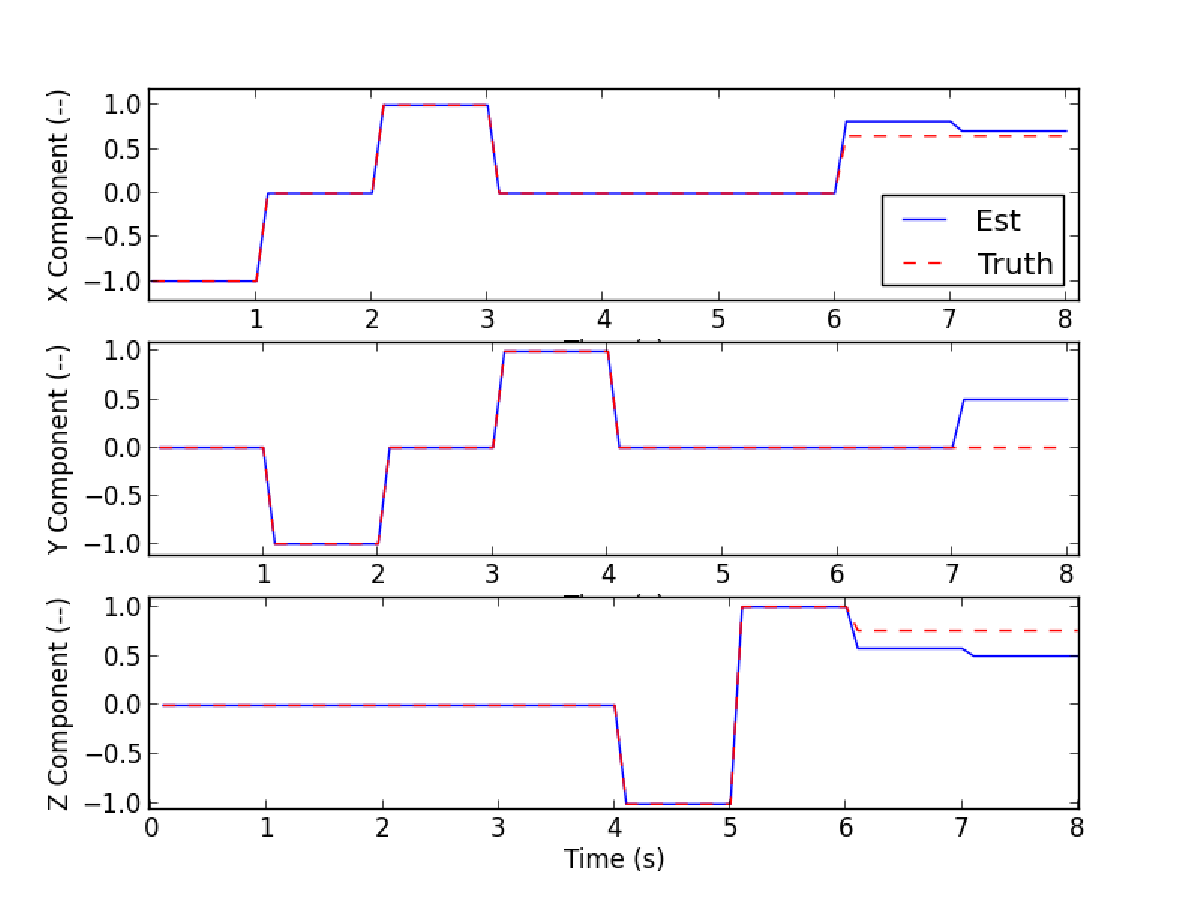
\includegraphics[scale=0.5]{Figures/sunEstAccuracy}
        }
        \caption{Truth and Estimated Sun Pointing Vector}
        \label{fig:point_fig}
\end{figure}

As this plot shows, the algorithm is very accurate up until 6.0 seconds, 
so both directions of the three primary body axes are estimated precisely.  
Then the double coverage case is reasonably accurate, but no longer precise as 
there isn't sufficient information available to get a good pointing direction.  
The single coverage test is not accurate at all (~45 degrees of error), but that 
is simply the best that the algorithm can do with that limited information.

Figure ~\ref{fig:num_fig} shows the number of CSSs used by the algorithm to 
estimate the sun pointing vector over the duration of the test.  It continues 
for longer than Figure~\ref{fig:point_fig} because the algorithm stops setting 
its output message once it gets to the zero valid sensors case as there is no 
good information to provide.
\begin{figure}[htb]
        \centerline{
        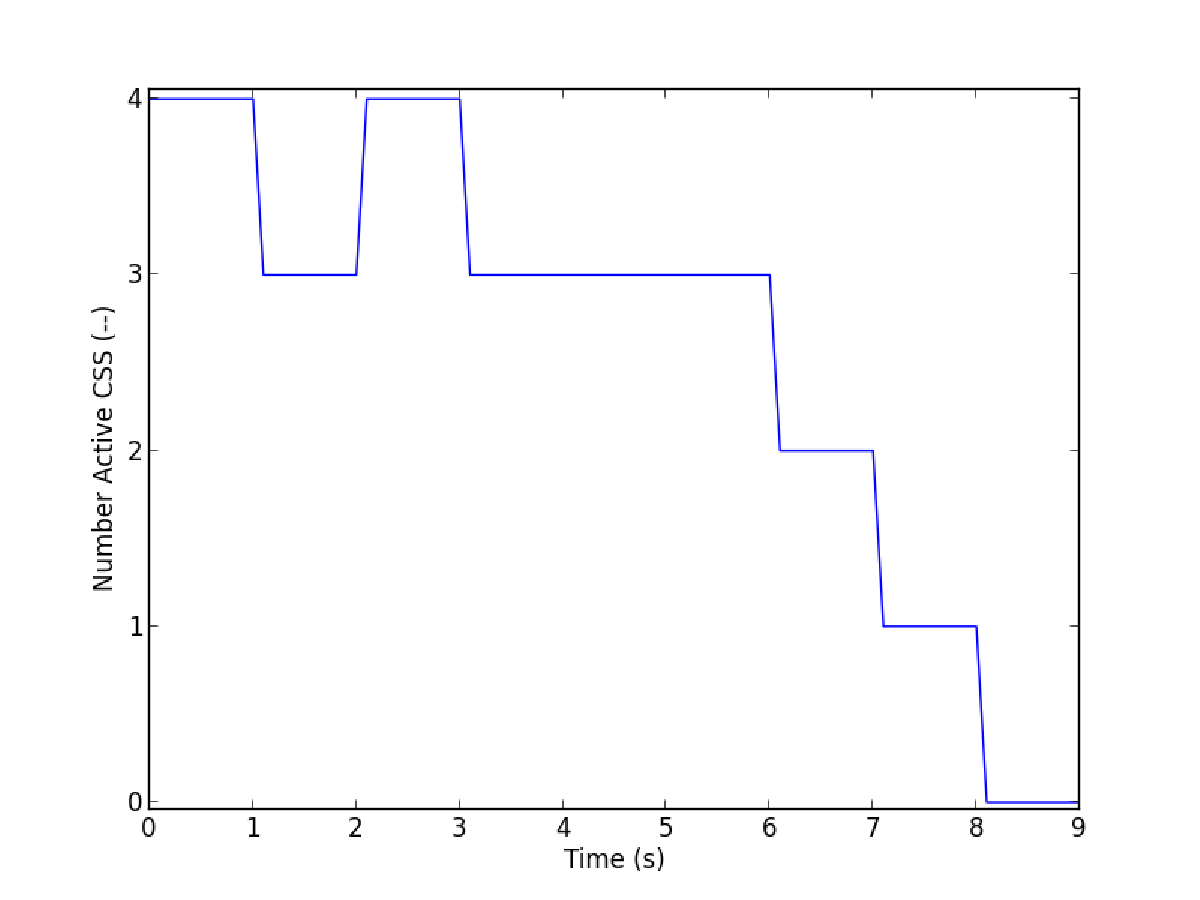
\includegraphics[scale=0.5]{Figures/numGoodCSS}
        }
        \caption{Number of CSSs Used in Estimate}
        \label{fig:num_fig}
\end{figure}


\begin{enumerate}
\item{Main Body Axis Estimates: The sun pointing estimation algorithm is not 
   required to provide a precise estimate of the Sun direction.  This algorithm 
   is only intended to be used in safe mode where the arrays only need to be 
   approximately pointed at the Sun.  For this reason, a pointing vector 
   was flagged as successful when it provided the Sun direction within 17.5 
   degrees which corresponds to a cosine loss of approximately 5\%.  All body 
   axes met this criteria with large margins.  A check was also performed that 
   verified that the predicted number of CSSs matched up with what the 
   algorithm used and this check was also 100\% successful.  The UseWeights flag 
   was initially set to False, and then was changed to True after two cases to 
   ensure that the algorithm works correctly in both cases. 
    \textcolor{ForestGreen}{Test successful.}}
\item{Double Coverage Test: The same accuracy criteria was used for this test.  
   This is mostly a function of CSS geometry and it is also the main driving 
   case for the success criteria used.  It was correct to within 14 degrees. 
   The predicted number of CSSs used (2) also matched the algorithm's selection. 
    \textcolor{ForestGreen}{Test successful.}}
\item{Single Coverage Test: The single coverage case did not have its accuracy 
   tested as there are no accuracy requirements for this case.  It simply must 
   provide an estimate and exit.  The predicted number of CSSs used (1) did  
   match the algorithm's selection.  \textcolor{ForestGreen}{Test successful.}}
\item{Zero Coverage Test: The zero coverage test is only provided here to 
   demonstrate that the algorithm passivates its outputs without hitting any 
   unacceptable event.  It does correctly flag that no valid CSSs were found 
   during the test. \textcolor{ForestGreen}{Test successful.}}
   
   \item{Angular Velocity Test:  The same 8 unit CSS configuration is used as in the earlier tests, but the true sun heading is set equal to $\hat{\bm b}_{1}$.  A BSK sample time of 0.5 seconds is setup, and the simulation is run 3 times to reach a simulation time of 1.0 seconds.  It takes 2 steps for the module to evaluate the update rate $\D t$, thus the expected rate estimate is a zero vector for these steps.  As the sun heading is being evaluated in the 2nd step, with the 3rd step there is a non-zero $\D t$ value, but the old and new sun-heading vectors are the same.  The expected rate output is again a zero vector.  Next the true sun heading is changed to be $\hat{\bm b}_{2}$, corresponding to a 90$\deg$ heading change about $\hat{\bm b}_{3}$.  The simulation is run for two more steps. The expected inertial body rate with step 4 would be $-\pi$ rad/sec about $\hat{\bm b}_{3}$.  The 5th step must yield again a zero rate vector as the sun heading has not changed.  Next, a reset function is called and a single simulation step is called.  The expected output is the zero rate vector again.  Finally, the true sun heading vector is changed back to $\hat{\bm b}_{1}$ and another simulation step is performed to show a $+\pi$ rad/sec rotation about $\hat{\bm b}_{3}$.  
   The test results status is: \input{AutoTeX/passFailRate.tex}}
\end{enumerate}

\section{Test Coverage}
The method coverage for all of the methods included in the cssWlsEst 
module are tabulated in Table~\ref{tab:cov_met}

\begin{table}[htbp]
    \caption{ADCS Coarse Sun Sensor Estimation Coverage Results}
   \label{tab:cov_met}
        \centering \fontsize{10}{10}\selectfont
   \begin{tabular}{c | r | r | r} % Column formatting, 
      \hline
      Method Name    & Unit Test Coverage (\%) & Runtime Self (\%) & Runtime Children (\%) \\
      \hline
      SelfInit\_cssWlsEst& 100.0 & 0.0 & 0.0 \\
      CrossInit\_cssWlsEst & 100.0 & 0.0 & 0.0 \\
      computeWlsmn & 100.0 & 0.01 & 0.64 \\
      Update\_cssWlsEst & 100.0 & 0.04 & 0.88 \\
      \hline
   \end{tabular}
\end{table}

For all of the code this test was designed for, the coverage percentage is 
100\%.  For Safe Mode, we do expect this algorithm to be the highest usage 
element from an ADCS perspective, so the CPU usage is almost certainly fine as 
is.  The main penalty comes from the use of matrix multiply in the computeWlsmn 
function.  The only issue of note here is that the matrix multiply algorithm(s) 
use in the FSW should be optimized as much as possible as they are major sources 
of CPU spin.

\section{Conclusions}
The safe mode sun vector estimator described in this document is functionally 
ready from a PDR perspective.  It has no noted failure cases, all code is tested 
for statement coverage, and it successfully meets its test criteria for all 
cases.  The only area where there might be a question is the desired behavior 
for zero-coverage cases.  We may wish to change the outputs to something more 
obviously in-error instead of just having the algorithm go silent.










%	
%% !TEX root = ./Basilisk-pixelLineConverter-20190524.tex


\begin{figure}[H]
	\centerline{
		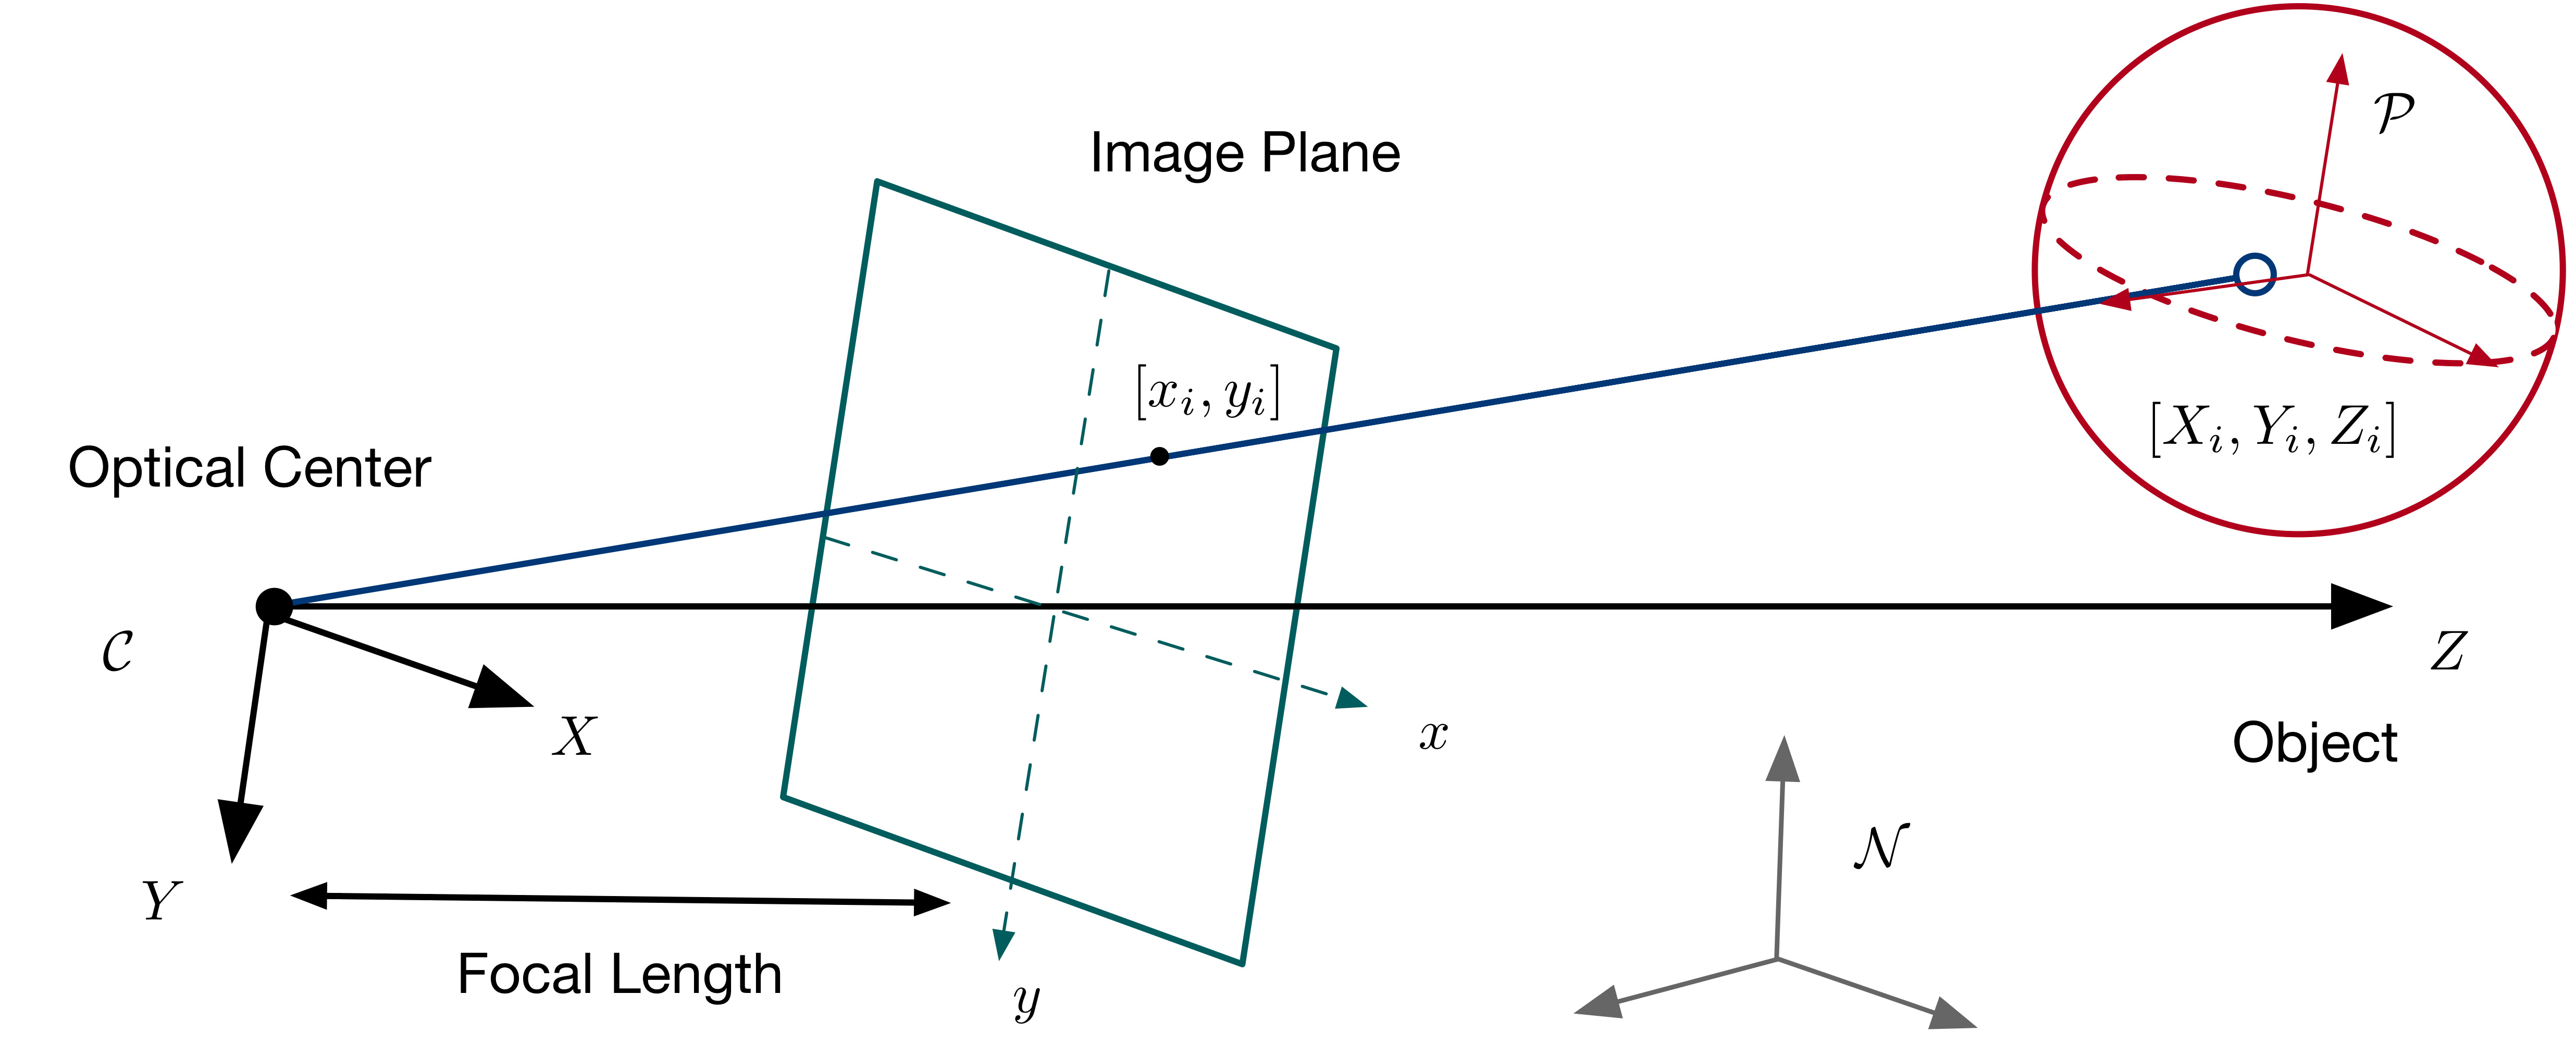
\includegraphics{Figures/CameraGeometry}
	}
	\caption{Camera Model}
	\label{fig:camera}
\end{figure}

\section{Model Description}

\subsection{Input and Output}

This converter module processes the output of a limb finding method to extract spacecraft inertial position. It does this by reading spacecraft attitude (coming from star tracker or other means), camera parameters, and the limb data. 

Messages read:

\begin{itemize}
\item CameraConfigMsg: containing focal length, resolution, and sensor size. These values are needed for the following computations. Notably the camera frame relative to the body frame is used.
\item LimbInMsg: Limb points, and uncertainty around these values in pixels. 
\item NavAttInMsg: Used for the spacecraft attitude. This allows to move from the body frame to the inertial frame.
\end{itemize}

Message written:
\begin{itemize}
\item OpNavFswMsg: Message containing $\leftexp{N}{\bm r}$ and it's covariance.
\end{itemize}

\subsection{Position computation}

The details of the algorithm are summarized in the papers attached. The engineering note contains a summary of the algorithms and covariance analysis. The journal paper \cite{Chirstian_Limb} contains the details of the development and assumptions. 

The component that is chosen in the implementation is the way to solve the least squares for equation $$[H] \bm x = \bm 1$$

This is done in this module by performing a QR-decomposition via a a Gram-Schmidt process. This leads to the following equation:

$$[R] \bm x = [Q]^T\bm 1$$

Since $[R]$ is upper-triangular, this is solved with an implemented back-substitution.  %This section includes mathematical models, code description, etc.
%
%% !TEX root = ./Basilisk-MODULENAME-yyyymmdd.tex


\section{Module Functions}
This module 
\begin{itemize}
	\item \textbf{Compute atmospheric density and temperature}: Each of the provided models is fundamentally intended to compute the neutral atmospheric density and temperature for a spacecraft relative to a body. These parameters are stored in the AtmoPropsSimMsg struct. Supporting parameters needed by each model, such as planet-relative position, are also computed.
	\item \textbf{Communicate neutral density and temperature}: This module interfaces with modules that subscribe to neutral density messages via the messaging system.
	\item \textbf {Subscribe to model-relevant information:} Each provided atmospheric model requires different input information to operate, such as current space weather conditions and spacecraft positions. This module automatically attempts to subscribe to the relevant messages for a specified model. 
	\item \textbf{Support for multiple spacecraft and model types} Only one Atmosphere module is required for each planet, and can support an arbitrary number of spacecraft. Output messages for individual spacecraft are automatically named based on the environment type.
\end{itemize}

\section{Module Assumptions and Limitations}
Individual atmospheric models are complex and have their own assumptions. At present, all non-exponential models are Earth-specific. For details about tradeoffs in atmospheric modeling, the reader is pointed to ~\citenum{vallado2013}.  %This includes a concise list of what the module does. It also includes model assumptions and limitations
%
%% !TEX root = ./Basilisk-thrFiringRemainder-2019-03-28.tex

\section{Test Description and Success Criteria}
The unit test creates a desired thruster force input vector and then runs the simulation for 3 seconds.  If the {\tt resetCheck} flag is true then a {\tt reset()} method is called and the simulation is repeated for another 2.5 seconds.  If the {\tt dvOn} flag is set than the off-pulsing mode is checked.  




\section{Test Parameters}

The simulation sets up 8 thrusters.  All permutations with the {\tt resetCheck} and {\tt dvOn} states are run.  The output is checked to the tolerance shown in Table~\ref{tab:errortol}.

\begin{table}[htbp]
	\caption{Error tolerance for each test.}
	\label{tab:errortol}
	\centering \fontsize{10}{10}\selectfont
	\begin{tabular}{ c | c } % Column formatting, 
		\hline\hline
		\textbf{Output Value Tested}  & \textbf{Tolerated Error}  \\ 
		\hline
		{\tt OnTimeRequest}        & 1e-05	   \\ 
		\hline\hline
	\end{tabular}
\end{table}




\section{Test Results}
All of the tests passed:
\begin{table}[H]
	\caption{Test results}
	\label{tab:results}
	\centering \fontsize{10}{10}\selectfont
	\begin{tabular}{c | c  | c } % Column formatting, 
		\hline\hline
		{\tt resetCheck} & {\tt dvOn} &\textbf{Pass/Fail} \\ 
		\hline
	   False & False	   			& \input{AutoTeX/passFailFalseFalse} \\ 
	   False & True	   			& \input{AutoTeX/passFailFalseTrue} \\ 
	   True & False	   			& \input{AutoTeX/passFailTrueFalse} \\ 
	   True & True	   			& \input{AutoTeX/passFailTrueTrue} \\ 
	   \hline\hline
	\end{tabular}
\end{table}



 % This includes test description, test parameters, and test results
%


\section{User Guide}

The model can be configured according to the user's wishes, but the following
rules of thumb should probably be respected unless the user is confident:
\begin{enumerate}
\item{The internal simulation dynamics step time should be less than or equal
     to the thruster ramp-up/ramp-down time steps}
\item{The internal simulation dynamics step time should be less than or equal to
     the desired thruster discretization level}
\item{The internal simulation dynamics step time should be less than one-tenth
    of the expected minimum allowable thruster firing duration}
\end{enumerate}

A common set up for thrusters, contains:

\begin{itemize}
  \item[-]      \texttt{thrusterSet = thrusterDynamicEffector.ThrusterDynamicEffector()}: Construct the Thruster Dyn Effector
  \item[-]   \texttt{thrusterSet.ModelTag = "ACSThrusterDynamics"}: Set the model tag
  \item[-]   \texttt{thruster1 = thrusterDynamicEffector.THRSimConfigMsgPayload()}: Create a individual thruster
  \item[-]   \texttt{thruster1.thrLoc\_B = [[1.0] ,[ 0.], [0.]] }: Set the thruster's location
  \item[-]   \texttt{thruster1.thrDir\_B = [[math.cos(anglerad)], [math.sin(anglerad)], [0.0]]}: Set the thruster thrust direction
  \item[-]   \texttt{thruster1.MaxThrust = 1.0}: Set the max thrust
  \item[-]   \texttt{thruster1.MaxSwirlTorque = 0.5}: Set the maximum swirl torque
  \item[-]   \texttt{thruster1.steadyIsp = 226.7}: Set the $I_{sp}$
  \item[-]   \texttt{thruster1.MinOnTime = 0.006}: Set the minimum on time
  \item[-]   \texttt{thrusterSet.addThruster(thruster1)}: Add thruster to the Dyn Effector
\end{itemize}

If attaching the thruster to a body, the last line is instead:

\begin{itemize}
     \item[-]   \texttt{thrusterSet.addThruster(thruster1, bodyStatesMsg)}: Add thruster to the Dyn Effector and attach it to a different body through the states message
\end{itemize}

If setting up a ramp, the user must also perform this:

\begin{itemize}
 \item[-]      \texttt{rampOnList = []}
 \item[-]      \texttt{rampOffList = []}

 \item[-]      \texttt{for i in range(rampsteps):}

\hspace{2cm}\texttt{fnewElement = thrusterDynamicEffector.THRTimePairSimMsg()}

\hspace{2cm}\texttt{fnewElement.TimeDelta = (i + 1.) * 0.1}

\hspace{2cm}\texttt{fnewElement.ThrustFactor = (i + 1.0) / 10.0}

\hspace{2cm}\texttt{fnewElement.IspFactor = (i + 1.0) / 10.0}

\hspace{2cm}\texttt{frampOnList.append(newElement)}

\hspace{2cm}\texttt{fnewElement = thrusterDynamicEffector.THRTimePairSimMsg()}

\hspace{2cm}\texttt{fnewElement.TimeDelta = (i + 1) * 0.1}

\hspace{2cm}\texttt{fnewElement.ThrustFactor = 1.0 - (i + 1.0) / 10.0}

 \hspace{2cm}\texttt{fnewElement.IspFactor = newElement.ThrustFactor}

 \hspace{2cm}\texttt{frampOffList.append(newElement)}

 \item[-]      \texttt{thrusterSet.thrusterData[0].ThrusterOnRamp =}

  \texttt{thrusterDynamicEffector.ThrusterTimeVector(rampOnList)}: Add the on ramp
 \item[-]      \texttt{thrusterSet.thrusterData[0].ThrusterOffRamp =}

 \texttt{thrusterDynamicEffector.ThrusterTimeVector(rampOffList)}: Add the off ramp
\end{itemize}

If setting up blow down effects, the user must also add these optional parameters to the thruster model before adding it to the set:

\begin{itemize}
  \item[-]   \texttt{thruster1.thrBlowDownCoeff = [1.0 , 2.0, 3.0] }: Set any number of polynomial coefficients for mass to thrust equation
  \item[-]   \texttt{thruster1.thrLoc\_B = [1.0 , 2.0, 3.0] }: Set any number of polynomial coefficients for mass to $I_{sp}$ equation
\end{itemize}
 % Contains a discussion of how to setup and configure  the BSK module






\bibliography{bibliography} %This includes references used and mentioned.

\end{document}
